% OTRec — NeurIPS 2026 submission
% Blind submission uses the default review mode below.
% For arXiv/preprint builds, switch to \usepackage[preprint]{neurips_2026}.
% For camera-ready, switch to \usepackage[main,final]{neurips_2026}.

\PassOptionsToPackage{numbers,compress}{natbib}
\documentclass{article}
\usepackage{neurips_2026}

\usepackage[utf8]{inputenc}
\usepackage[T1]{fontenc}
\usepackage{amsmath,amssymb}
\usepackage{booktabs}
\usepackage{graphicx}
\usepackage{url}
\usepackage{xcolor}
\usepackage{microtype}
\usepackage{nicefrac}
\usepackage{hyperref}

\title{OTRec: A Deep Learning Recommender for\\
Druggable Disease--Target Prioritization}

\author{Anonymous Authors}

\begin{document}
\maketitle

\begin{abstract}
Identifying druggable disease--target associations remains a central
challenge in translational medicine, limiting therapeutic discovery and repurposing.
Here, we present OTRec, a deep learning--based recommender system that
ranks such associations at scale and evaluates them in a 
temporal hold-out setting.
Unlike approaches that rely on manually curated or aggregated evidence
scores, OTRec employs a two-tower architecture to learn latent
representations from $663{,}351$ disease--target pairs.
The model integrates heterogeneous inputs, including textual
descriptions, ontology-derived features, and biological annotations
such as tractability, Gene Ontology terms, and pathway information.
We perform temporal validation by training on the 2022 Open
Targets release and evaluating on clinical trial data from 2025.
OTRec improves on the retrospective Open Targets association
score on ROC-AUC ($0.863$ vs.\ $0.558$); on PR-AUC it is comparable to
a target-prior baseline ($0.303$ vs.\ $0.293$, gap $0.010$).
Using $5{\times}5$ target-disjoint cross-validation, OTRec reaches
ROC-AUC $0.950$ (PR-AUC $0.844$), narrowly improving on the same-feature
CatBoost baseline.
At inference we rank the druggable genome across ${\sim}19{,}000$
OTP diseases and release ${\sim}282{,}500$ candidate associations
above a $0.65$ score threshold (in-distribution CV precision $0.92$;
out-of-distribution precision not directly estimated), covering
$4{,}346$ diseases including $2{,}322$ orphan diseases, through
an interactive prediction platform.
Code, weights, ranked predictions, and the interactive demo are publicly available: [anonymized during review period].
\end{abstract}

% -----------------------------------------------------------------------
\section{Introduction}
% -----------------------------------------------------------------------

Drug discovery is hindered by a pervasive ``streetlight effect'':
research concentrates on well-studied targets while large regions of
the druggable genome remain under-investigated~\citep{buniello2025,richardson2023understudied,harel2018}.
The Open Targets Platform (OTP) integrates diverse evidence sources---from
GWAS associations to text-mined literature---but the resulting association
scores are intrinsically retrospective, reflecting existing knowledge
rather than a target's prospective therapeutic promise.
A zero or low score may signal an absence of investigation rather than a
genuine lack of relevance.
Moreover, manually designed, rule-based scoring frameworks typically
underperform relative to data-driven, learned approaches~\citep{ulain2015mlscoring}.

We therefore developed \textbf{OTRec} (Open Targets Recommender).
The task is: given a disease, rank every gene in the druggable
genome by its probability of entering clinical trials---a label OTP
 captures across ${>}17{,}000$ diseases.
In this work, ''target'' denotes an OTP gene target (mapped to Ensembl gene IDs),
and ''drug'' denotes therapeutic evidence represented in OTP via approved or
clinical-stage associations linked to those targets.
Unlike OTP's rule-based aggregations~\citep{han2022}, OTRec uses a
two-tower neural architecture that separately encodes disease and target
representations from raw biomedical text and ontology. These representations
are scored by cosine similarity, which natively enables attribute-cold-start
inference for targets absent from training folds but still represented
through public annotations.
Validated in a temporal hold-out against later trial entries, it improves on the
retrospective OTP score and learned baselines in target-disjoint CV,
and we release ${\sim}282{,}500$ candidate associations above a
$0.65$ score threshold with a fully interactive platform.

Our contributions are threefold:
(i) a two-tower neural recommender that learns disease and target
representations from raw biomedical text and ontology, supporting
attribute-cold-start prediction for novel, annotated targets;
(ii) a temporal-hold-out benchmark that combines target-disjoint CV with a
2022$\to$2025 temporal split on the OTP target-prioritization task,
on which OTRec improves on the retrospective OTP score while remaining
competitive with OTP-native tree baselines; and
(iii) a public, ranked candidate dataset of ${\sim}282{,}500$ novel
disease--target associations covering $4{,}346$ diseases (including
$2{,}322$ orphan diseases) with an interactive query interface.

% -----------------------------------------------------------------------
\section{Related Work}
\label{sec:related}
% -----------------------------------------------------------------------

Disease--target prioritization sits between recommendation,
biomedical knowledge integration, and drug--target interaction (DTI)
prediction. We organize prior work into four threads and explain why
none directly address prospective target prioritization on OTP.

\textbf{OTP-native ML.}
The closest prior work, Han et al.~\citep{han2022}, trains gradient
boosting on $14$ OTP evidence-channel features and is the strongest
publicly reimplementable baseline we can include in our benchmark.
It inherits the retrospective bias of OTP evidence channels, which is
precisely what our temporal evaluation is designed to expose.

\textbf{Knowledge-graph and graph neural network DTI.}
KG embedding and GNN methods, such as DRKG and KGNN-LS,
integrate heterogeneous biomedical entities and relations~\citep{ratajczak2022taskdriven,wang2019kgnnls,nicholson2020}.
These methods rely on a pre-curated interaction graph whose edges
themselves encode the same investigation bias we aim to escape.
Furthermore, they are typically evaluated on curated DTI benchmarks (BindingDB, DAVIS) with
balanced positive/negative ratios, and do not natively support the
OTP implicit-feedback, target-disjoint, time-split regime.
We include Matrix-Factorization and TF-IDF controls that serve as
comparable cold-start relational baselines.

\textbf{Chemistry-centric DTI.}
Deep DTI models such as DeepPurpose and MolTrans and related transformer
approaches~\citep{huang2020,huang2021moltrans} predict binding affinity from compound
structure and protein sequence. Their inputs (SMILES, sequence) and
labels (binding affinity) are orthogonal to the disease-level clinical
relevance signal modeled here, so they cannot be evaluated on the
same benchmark without redefining the task.

\textbf{Biomedical text encoders and prospective benchmarks.}
Biomedical language models (BioBERT, PubMedBERT~\citep{gu2021}) and
benchmarking suites such as Therapeutics Data Commons~\citep{huang2021tdc}
provide reusable text representations and standardized splits, respectively.
Neither defines a disease--target prioritization task with
prospective clinical-trial-entry labels at OTP scale; we introduce
this benchmark and release splits, code, and candidate predictions
to enable direct replication and comparison.

% -----------------------------------------------------------------------
\section{Methods}
\label{sec:methods}
% -----------------------------------------------------------------------

\subsection{Problem Formulation and Data}

We formulate target prioritization as an implicit-feedback recommendation
task: rank candidate human protein-coding genes for a given disease by
likelihood of clinical relevance.
Positive labels ($y{=}1$) are disease--target pairs with evidence of
clinical progression (clinical trials or approved drugs) in
OTP Release 2025.06; all remaining pairs are implicit negatives
($y{=}0$).
The implicit-feedback formulation conflates true negatives with unlabeled
positives; we treat this label noise as inherent to the prospective task.
The temporal split (\S\ref{sec:eval}) provides a partial empirical bound
by re-labeling pairs that subsequently progressed to trials.

\textbf{Scope of ``drug'' and ``gene''.}
Throughout, ``drug'' follows OTP usage and covers any therapeutic entity
in the OTP drug index ($N{=}18{,}081$ entities in Release 2025.06,
of which $10{,}956$ have reached clinical phase~${\geq}1$):
small molecules ($N{=}14{,}848$, $82\%$ of the index), antibodies
($N{=}963$), proteins / peptides / enzymes ($N{=}830$),
oligonucleotides ($N{=}159$), antibody--drug conjugates ($N{=}119$),
gene therapies ($N{=}117$), cell therapies ($N{=}52$), and vaccines.
``Gene'' / ``target'' refers to the human protein-coding subset of
the Finan et al.\ druggable genome~\citep{finan2017} (${\sim}4{,}600$
genes, of $20{,}130$ protein-coding genes in OTP).
Non-coding loci catalogued by OTP (lncRNAs $N{=}34{,}882$, miRNAs
$N{=}1{,}879$, snRNAs, pseudogenes) are excluded from both the
training label set and the inference pool, mirroring the
small-molecule / biologic-modality bias of the OTP drug index;
we revisit this scope in~\S\ref{sec:limitations}.

We applied filtering criteria aligned with prior work~\citep{han2022}:
non-specific ontology terms (``measurement'', ``phenotype'', ``biological
process'', ``cell proliferation disorder'') were excluded.
Training restricts to ${{\sim}}1{,}500$ targets with clinical associations
across any indication, excluding targets with only a single-disease
evidence record to reduce disease-specific overfitting.
The training set comprises 663{,}351 disease--target pairs spanning
${\sim}6{,}000$ positive-bearing diseases (out of ${>}12{,}000$
diseases overall in the training pool; 67{,}532 positives, 10\%).
During inference, the model ranks the full druggable
genome~\citep{finan2017} (${\sim}4{,}600$ genes) across
${\sim}19{,}000$ valid OTP diseases.
Note that CV metrics characterise generalization within the
multi-indication-clinical training subset and should be read as an
upper bound on full-druggable-genome inference quality.

\subsection{Model Architecture and Features}

OTRec uses a multi-input two-tower architecture (Figure~\ref{fig:model}A)
that separately encodes disease and target representations, enabling the
model to learn semantic and biological similarities from text and
ontology structure.

\textbf{Inputs.}
Text features are processed via Text Vectorization (bag-of-words, count
mode).
The \emph{disease tower} uses disease names, descriptions, exact synonyms,
therapeutic areas, phenotypes, and ontology parents (EFO terms),
concatenated with a learned disease-ID embedding ($d{=}64$).
The \emph{target tower} uses gene symbol, name, synonyms, function
descriptions, Gene Ontology terms, pathway annotations, and tractability
features including genetic constraint scores.

\textbf{Architecture and training.}
Each tower applies a Residual ``Wide \& Deep'' block: a direct linear
projection ($d{=}384$) summed with a nonlinear bottleneck path
(Dense $384{\to}64{\to}384$, ELU activations, Dropout $0.15$--$0.35$).
The 384-dimensional embeddings interact via normalized dot product
(cosine similarity), followed by a multi-task head: a sigmoid output
predicts clinical trial entry while an auxiliary linear head predicts
the OTP overall association score from the same release used to
construct the training split (2025.06 in target-disjoint CV, 2022.02
in the temporal experiment).
In the temporal experiment, the auxiliary target is the 2022.02 OTP
overall score, so the model does not use post-cutoff information.
Training used Adam (LR $8{\times}10^{-3}$, batch size $1{,}024$) with
dynamic LR annealing and early stopping on a held-out 5\% validation
set.
Implementation: TensorFlow/Keras~\citep{chollet2015}.

\subsection{Evaluation and Baselines}
\label{sec:eval}

\textbf{Target-disjoint CV.}
To evaluate generalization to novel targets unseen during training, we
use $5{\times}5$-fold target-disjoint cross-validation ($5$ folds,
$5$ repeats, $25$ folds total).
In each fold, $20\%$ of targets are withheld; all associations involving
held-out targets are removed from training.
This is attribute-cold-start rather than annotation-free cold-start:
held-out targets remain represented by public text, ontology, pathway,
and tractability features.

\textbf{Temporal split.}
A model trained on OTP Release 2022.02 is tested on pairs with no
clinical evidence in 2022 that entered clinical trials by 2025.
The test set covers ${\sim}12{,}000$ diseases (vs.\ ${\sim}6{,}000$
positive-bearing diseases at training time), making it strongly
covariate-shifted in both disease coverage and label distribution.
Any 2025 positive whose earliest trial start predated 2022.02 is
excluded to prevent leakage.

\textbf{Baselines.}
We benchmark against six methods spanning ML, ontology-aware, and
cold-start controls:
(\textit{i})~\textbf{OTTree}: CatBoost~\citep{dorogush2018} trained on
the same OTRec feature set, isolating the contribution of the
two-tower architecture from the feature engineering;
(\textit{ii})~\textbf{Han et al.}~\citep{han2022}: XGBoost on the
$14$ OTP evidence-channel scores (genetic association, somatic
mutation, known drug, affected pathway, RNA expression, literature,
animal models, etc.), the strongest publicly reimplementable ML
baseline for the OTP target-prioritization task;
(\textit{iii})~\textbf{Open Targets Score}: the raw OTP overall
association score (which itself aggregates clinical evidence and is
therefore an upper bound on retrospective performance);
(\textit{iv})~\textbf{Target Mean}: the per-target positive rate
computed on the training split, broadcast to every candidate disease
for that target (a strong historical-frequency prior);
(\textit{v})~\textbf{Matrix Factorization}: TruncatedSVD on the
binary positive interaction matrix;
(\textit{vi})~\textbf{TF-IDF cosine}: lexical similarity between
concatenated disease and target text fields.
The last two are cold-start controls verifying that the
target-disjoint regime is non-trivial.

% -----------------------------------------------------------------------
\section{Results}
\label{sec:results}
% -----------------------------------------------------------------------

\begin{figure}[t]
  \centering
  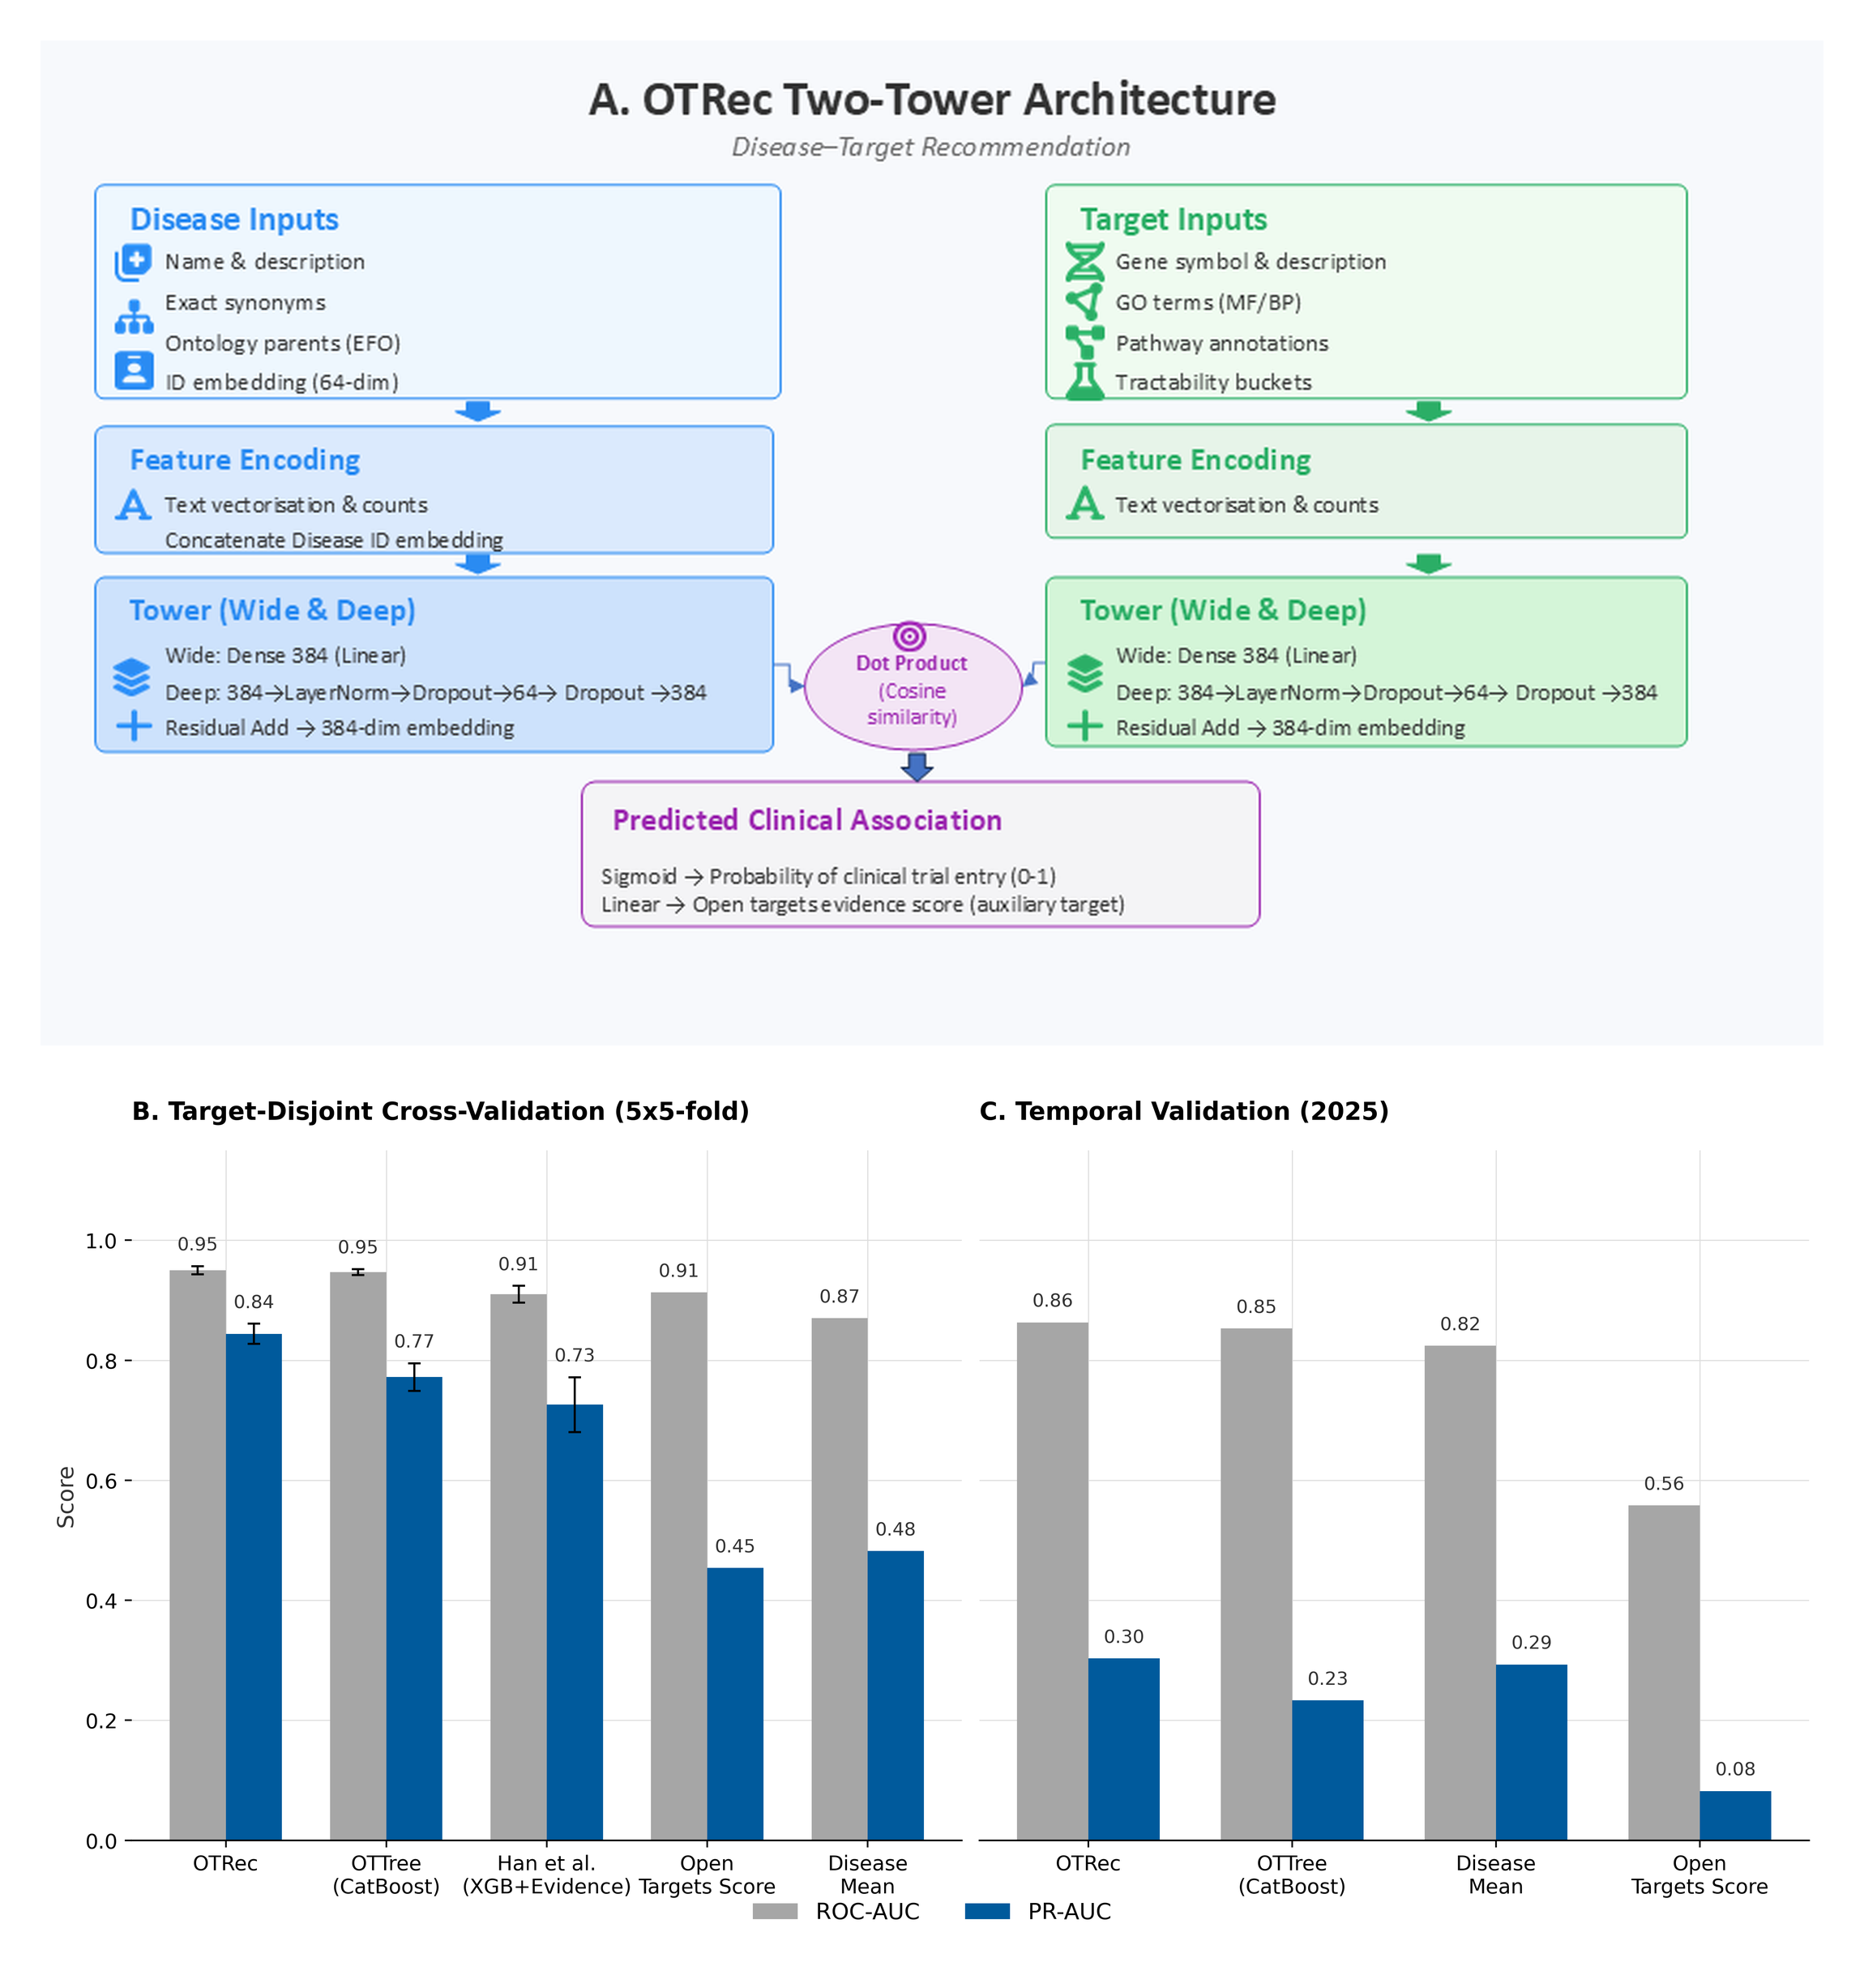
\includegraphics[width=\linewidth]{media/image1.png}
  \caption{
    \textbf{OTRec architecture and performance.}
    \textbf{(A)} The two-tower model separately encodes disease and
    target features (text, ontology, tractability, gene symbol/name) into
    384-dimensional embeddings compared by normalized dot product
    (cosine similarity) to predict clinical trial entry probability.
    \textbf{(B)} Target-disjoint $5{\times}5$ cross-validation results.
    OTRec achieves the highest mean ROC-AUC ($0.95$) and
    PR-AUC ($0.844$); error bars denote standard deviation.
    \textbf{(C)} Temporal hold-out validation (training on 2022,
    predicting 2025 entries). Panel C shows single-model point
    estimates only; no confidence intervals are available.
  }
  \label{fig:model}
\end{figure}

\subsection{Benchmark Comparison}

In the $5{\times}5$ target-disjoint CV (Table~\ref{tab:cv}), OTRec
achieves ROC-AUC $0.950$ (PR-AUC $0.844$), marginally surpassing
OTTree ($0.947$ / $0.772$) and exceeding the Open Targets
Score ($0.913$ / $0.454$).
Because Han et al. uses only $14$ OTP evidence channels whereas OTRec
and OTTree use the richer text+ontology+tractability feature set,
OTRec's gain over Han et al. reflects both feature engineering and model
class. The OTRec--OTTree gap isolates the two-tower contribution on
matched inputs ($+0.003$ ROC-AUC).
The large gap between OTRec and cold-start controls
(Target Mean: $0.870$; Matrix Factorization: $0.811$; TF-IDF: $0.513$)
indicates that the target-disjoint regime genuinely tests generalization
to novel targets, and that OTRec's advantage comes from learned
biological content transfer rather than interaction memorization or
surface text matching.

In the temporal setting (Table~\ref{tab:temporal}), OTRec improves over
the retrospective OTP score on ROC-AUC by $0.305$ ($0.863$ vs.\
$0.558$), while achieving PR-AUC ($0.303$) comparable to the stronger
historical Target Mean prior ($0.293$, gap $0.010$) and well above a
disease-only prior ($0.052$).
Fast cold-start controls are substantially weaker in this prospective
regime (Matrix Factorization: $0.553$ / $0.050$; TF-IDF cosine:
$0.512$ / $0.042$), indicating that historical priors and learned
representations carry most of the forward signal.
Historical target-level priors carry real prospective signal; OTRec's
advantage over them is concentrated in pair-level ranking (ROC-AUC),
not in simply recovering which targets already accumulated many known
indications.
The temporal model uses the 2022.02 OTP overall score for both its
auxiliary target and the OTP-score baseline.

\begin{table}[t]
\caption{Benchmark performance in $5{\times}5$ target-disjoint
cross-validation (mean $\pm$ SD over 25 folds). A horizontal rule
separates ML baselines from cold-start controls.}
\label{tab:cv}
\centering\small
\setlength{\tabcolsep}{5pt}
\begin{tabular}{@{}lrrrr@{}}
\toprule
Model & ROC-AUC & ${\pm}$SD & PR-AUC & ${\pm}$SD \\
\midrule
\textbf{OTRec (ours)}  & \textbf{0.950} & 0.007 & \textbf{0.844} & 0.017 \\
OTTree (CatBoost)      & 0.947 & 0.005 & 0.772 & 0.023 \\
Han et al.\ (2022)     & 0.910 & 0.014 & 0.726 & 0.046 \\
\midrule
Open Targets Score     & 0.913 & ---   & 0.454 & ---   \\
Target Mean            & 0.870 & ---   & 0.482 & ---   \\
Matrix Factorization   & 0.811 & 0.008 & 0.265 & 0.014 \\
TF-IDF cosine          & 0.513 & 0.016 & 0.106 & 0.009 \\
\bottomrule
\end{tabular}
\end{table}

\begin{table}[t]
\caption{Temporal hold-out validation: trained on OTP 22.02, tested
on pairs with no 2022 clinical evidence that entered trials by OTP 25.06.
Values are single-model point estimates with no confidence intervals.}
\label{tab:temporal}
\centering\small
\begin{tabular}{@{}lrr@{}}
\toprule
Model & ROC-AUC & PR-AUC \\
\midrule
\textbf{OTRec (ours)} & \textbf{0.863} & \textbf{0.303} \\
OTTree (CatBoost)     & 0.853 & 0.233 \\
Target Mean           & 0.824 & 0.293 \\
Matrix Factorization  & 0.553 & 0.050 \\
TF-IDF cosine         & 0.512 & 0.042 \\
Disease Mean          & 0.593 & 0.052 \\
Open Targets Score    & 0.558 & 0.082 \\
\bottomrule
\end{tabular}
\end{table}

\subsection{Disease-Centric Shortlist Utility}

Aggregate ROC-AUC and PR-AUC measure pairwise discrimination, but
operational target prioritization is shortlist-driven: a curator
typically inspects only the first few predictions per disease.
We re-analysed target-disjoint out-of-fold predictions
disease-by-disease, restricting to the 2{,}329 diseases with at least
one held-out positive target (Table~\ref{tab:shortlist}).

OTRec placed a true positive at rank 1 for $68.2\%$ of diseases
(vs.\ $48.7\%$ for OTTree) and improved mean reciprocal rank
($0.741$ vs.\ $0.600$).
At rank 5, the advantage remained ($80.6\%$ vs.\ $73.2\%$); at rank 10
the two methods tied ($84.8\%$ each), and OTTree won at rank 25
($95.1\%$ vs.\ $89.7\%$).
At the same shortlist depth, OTRec also improved mean precision@5
($64.5\%$ vs.\ $53.7\%$) and mean recall@5 ($32.1\%$ vs.\ $27.2\%$).
OTRec is preferable for top-1 / top-5 curator workflows that surface a
short actionable shortlist; OTTree is preferable for broader screens
at $k{\geq}25$ where its more diffuse predictive distribution
recovers more positives.

\begin{table}[ht]
\caption{Disease-centric shortlist utility across 2{,}329 diseases with
${\geq}1$ held-out positive target.}
\label{tab:shortlist}
\centering\small
\begin{tabular}{@{}lrrrrrrr@{}}
\toprule
Model & Hit@1 & Hit@5 & P@5 & R@5 & Hit@10 & Hit@25 & MRR \\
\midrule
\textbf{OTRec}     & \textbf{68.2\%} & \textbf{80.6\%} & \textbf{64.5\%} & \textbf{32.1\%} & 84.8\% & 89.7\%          & \textbf{0.741} \\
OTTree (CatBoost)  & 48.7\%          & 73.2\%          & 53.7\%          & 27.2\%          & 84.8\% & \textbf{95.1\%} & 0.600 \\
\bottomrule
\end{tabular}
\end{table}

\subsection{Disease Repurposing Candidates}

We identified ${\sim}282{,}500$ candidate associations above a $0.65$
score threshold for $4{,}346$ diseases matched with $2{,}808$ targets,
including $2{,}322$ orphan diseases, where ``orphan'' here refers to
OTP diseases with no clinically associated target in 2025.06 rather
than a formal prevalence-based regulatory definition.
Candidates were generated by screening the druggable genome, removing
known links, and retaining predictions with score ${>}0.65$---a
threshold selected by inspecting the precision-recall curve on
out-of-fold CV data ($92\%$ in-distribution precision, $62\%$ recall;
up to 200 per disease).
Out-of-distribution precision for genuinely novel pairs is lower
and not directly estimated; the ranked prediction set should not be treated as a validated discovery list.
Predictions were further ranked and annotated using the InterFeat
framework~\citep{ofer2025};
full candidates are available in the
repository (supplementary text S1).
The interactive platform filters out known disease--target pairs, so
known associations are intentionally absent.

We additionally release an interactive Gradio web demo
(Figure~\ref{fig:gradio}) that lets users issue both forward (disease
$\to$ ranked targets) and reverse (target $\to$ ranked diseases) queries
against the trained model, with one-click links to the OTP and EFO
or ontology records when available, tractability annotations, packaged
comparison labels, and CSV export of the full
druggable-genome ranking.

\begin{figure}[t]
  \centering
  \IfFileExists{media/gradio_app.png}{%
    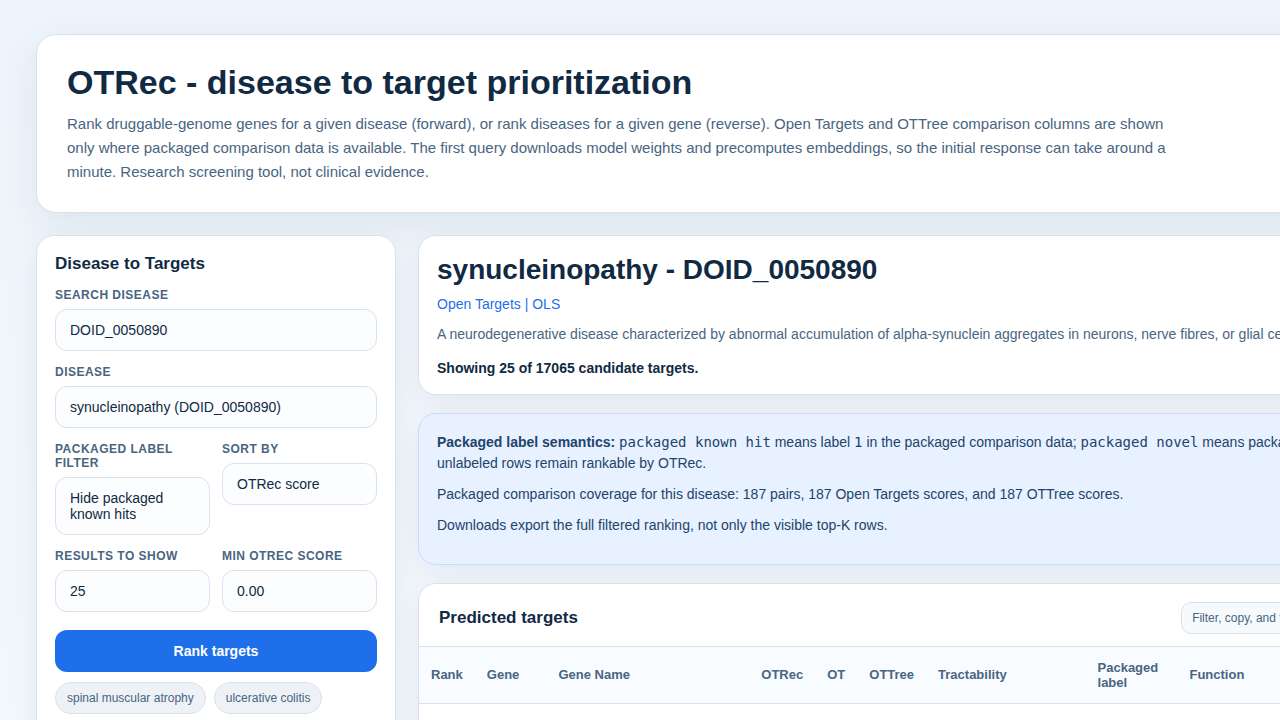
\includegraphics[width=0.95\linewidth]{media/gradio_app.png}%
  }{%
    \fbox{\parbox{0.9\linewidth}{\centering\vspace{1.5em}%
    \textit{[Gradio app screenshot placeholder --- add \texttt{media/gradio\_app.png}]}%
    \vspace{1.5em}}}%
  }
  \caption{\textbf{OTRec interactive demo.} Users select a
  disease or target; the Gradio app returns the ranked
  candidate list with OTP/EFO cross-links where supported, tractability
  category, and a CSV export of the full druggable-genome ranking.}
  \label{fig:gradio}
\end{figure}

\subsection{Selected Discovery Examples}

The following examples are illustrative of the candidates the
model ranks highly; they are not part of a systematic screen, are not
experimentally validated, and are outside the quantitative evaluation.
Full ranked lists are released with the dataset.

\paragraph{Temporal hold-out example: \textit{POLA1} / \textit{POLA2} in central nervous system cancer (2022$\to$2025).}
OTRec ranked the catalytic and
accessory subunits of replicative DNA polymerase~$\alpha$ ---
\textit{POLA1} (score $0.961$) and \textit{POLA2} (score $0.966$) ---
among the top candidates for central nervous system cancer
(EFO\_0000326), despite a near-zero OTP known-drug score in 2022
(${\sim}0.06$).
By the OTP 2025 release both pairs had crossed the
clinical-progression threshold ($y{=}1$ in our temporal test set),
coincident with inhibitors of the POL$\alpha$/primase complex entering
brain-tumour trials.

\paragraph{Spinal muscular atrophy (SMA).}
SMA is caused primarily by insufficient SMN protein from \textit{SMN1}
loss, and current therapies target SMN1/SMN2 biology.
OTRec nevertheless ranked ion-channel and synaptic-signaling candidates,
including potassium voltage-gated channel family members and
\textit{GABBR1}.
These predictions should be read as hypothesis-generating symptomatic
or modifier targets rather than disease-causal replacements for SMN
restoration: they point to neuronal excitability and inhibitory
signaling as possible complementary axes for model-system follow-up.

\paragraph{Croup and Coxsackievirus.}
OTRec ranked FKBP1A, an immunophilin co-opted by viral replication
complexes, among the top candidates; further rationale is documented
in the repository.

\paragraph{Limited cutaneous systemic sclerosis.}
PDE4C was ranked highly as a mechanism-based repurposing candidate;
apremilast (a PDE4 inhibitor) is already approved for related
indications.

\paragraph{Ulcerative colitis.}
OTRec ranked IL6R highly; clinical context for IL6-axis blockade in
UC is documented in the repository.

\subsection{Feature Contributions and Model Characteristics}
\label{sec:char}

\textbf{Characterization of novel predictions.}
Novel predicted targets (lacking approved drugs) are less genetically
constrained ($P < 3.3 \times 10^{-19}$, Cohen's $d{=}{-}0.37$) and
enriched for secreted proteins ($+8.4\%$, $P < 2.1 \times 10^{-7}$),
indicating divergent tractability profiles.
They map to significantly fewer annotated pathways
($P < 7.2 \times 10^{-50}$), reflecting lower annotation coverage
rather than functional irrelevance.
Paralog counts and sequence identity do not differ significantly
($P{=}0.63$), so this analysis does not suggest that OTRec is merely
prioritizing homologs of known genes.
The model assigns higher confidence to disease-specific targets
(median $0.936$) vs.\ multi-disease hubs (median $0.878$;
$P < 6.3 \times 10^{-17}$), consistent with mechanistic specificity;
representative high-degree hubs include GUCY1B2, tubulins, FKBP1A, and
DNA maintenance proteins such as POLD2.
This pattern is consistent with OTRec ranking pathway- or system-level
intervention points shared across diseases rather than only causal-gene
recovery, though such candidates still require experimental validation.
Comparing out-of-fold prediction scores against the maximum clinical
phase (1--4) reached by ${\sim}65{,}000$ known positive associations,
we observe a weak but significant positive correlation
(Spearman $\rho{=}0.20$), consistent with OTRec assigning higher
scores to candidates that progress to later development stages.
All p-values reported in this section are Bonferroni-corrected for the
six tests performed.

% -----------------------------------------------------------------------
\section{Limitations}
\label{sec:limitations}
% -----------------------------------------------------------------------

\textbf{Auxiliary supervision and objective dependence.}
The auxiliary head regresses the OTP overall association score from the
same release as each training split (2025.06 in CV; 2022.02 in the
temporal run), so the temporal experiment does not use post-cutoff 2025
supervision. The reported temporal point estimate uses a multi-task
objective rather than a pure binary objective.
An auxiliary-free temporal ablation would isolate how much the score
head changes optimization.

\textbf{Single temporal split.}
The 2022$\to$2025 evaluation uses one release pair and one trained
model, so temporal metrics carry no confidence intervals.
Bootstrap confidence intervals and rolling splits (e.g., 2021$\to$2024)
would substantially strengthen this claim and are direct next steps.

\textbf{Illustrative discovery examples.}
The four discovery cases are curated to span disease classes; they
are not the output of a systematic screen and have not been
experimentally validated. The full unfiltered candidate set is
released precisely to allow independent, unsupervised evaluation.

\textbf{Bag-of-words text encoding.}
We use count-mode text vectorization rather than a biomedical
transformer encoder (BioBERT, PubMedBERT). This trades representational
richness for inference scale (${\sim}87$M pairs at prediction time)
and interpretability of contributing tokens. Substituting a frozen
biomedical LM into either tower is a natural extension we did not
benchmark here.

\textbf{Implicit-feedback / PU formulation.}
All non-clinical pairs are treated as $y{=}0$; no positive-unlabeled
correction (Elkan--Noto, nnPU) is applied. The temporal split
partially calibrates this by relabeling pairs that entered trials
between 2022 and 2025, making the label-noise assumption testable
rather than purely assumed.

\textbf{Druggable-genome inference scope.}
Inference is restricted to the Finan et al.~\citep{finan2017}
druggable genome (${\sim}4{,}600$ protein-coding genes) and to
OTP-defined diseases. Non-coding targets (lncRNA, miRNA), intrinsically
disordered regions, and rare diseases without OTP records are outside
the released candidate set. OTRec also ranks targets independently and
does not model multi-target / off-target liabilities; downstream
polypharmacology and selectivity filters remain the curator's
responsibility.

\textbf{Population and disease-class bias.}
OTP over-represents European-ancestry GWAS cohorts and common
cardio-oncology indications. OTRec inherits these biases directly;
prediction calibration for under-represented populations and rare
conditions is likely lower than overall metrics imply.
Ancestry-stratified and indication-stratified validation are
necessary before acting on any candidate in those settings.

% -----------------------------------------------------------------------
\section{Conclusion}
% -----------------------------------------------------------------------

Ranking all druggable targets across all OTP diseases against future
clinical-trial entries is a tractable, precisely defined surrogate for
prospective therapeutic relevance, and one where learned representations
from text and ontology improve over the retrospective evidence score on
ROC-AUC, while PR-AUC matches a strong historical target-prior baseline.
OTRec makes this ranking available at scale: ${\sim}282{,}500$
candidate associations above a $0.65$ score threshold, an interactive
query interface, and a temporal benchmark against which
future models can be directly compared.
Rolling release splits, bootstrapped temporal CIs, and transformer-based
tower encoders are the natural next steps to test whether deeper
language representations extend the prospective advantage beyond the
BoW ceiling established here.

% -----------------------------------------------------------------------
\section*{Availability}
% -----------------------------------------------------------------------

The full artifact bundle (code, model weights, ranked predictions, and
the interactive query interface) will be released upon acceptance.
Reviewer access and launch instructions are provided via the
supplementary materials.

% -----------------------------------------------------------------------
\bibliographystyle{plainnat}
\bibliography{refs}

\appendix
\section*{Supplementary Material}
\label{sec:supp}

\textbf{S1.\ Full candidate predictions.}
The complete set of $\sim$282{,}500 novel disease--target candidates
(score${>}0.65$) for $4{,}346$ diseases, with InterFeat re-ranking
features, is released as
\texttt{Outputs/S1-DL\_novel\_predictions.csv} in the anonymized
repository.

\textbf{S2.\ Top novel and known candidates.}
\texttt{Outputs/S2-DL\_novel+known\_candidates.csv} contains the
top-50 novel and known disease--target candidates per disease,
intended for direct curatorial inspection.

\textbf{S3.\ Per-feature-group ablation.}
A per-feature-group ablation table (text-only, +ontology, +tractability,
$-$auxiliary head) is provided in the repository under
\texttt{Outputs/CV\_DL/}.

\textbf{S4.\ Baseline reproduction.}
Matrix Factorization, TF-IDF, and Han-style XGBoost baselines can be
reproduced via \texttt{baselines/run\_baselines.py}; per-fold metrics
are in \texttt{Outputs/CV\_baselines/}.

\section*{NeurIPS Paper Checklist}

\begin{enumerate}

\item {\bf Claims}
    \item[] Question: Do the main claims made in the abstract and introduction accurately reflect the paper's contributions and scope?
    \item[] Answer: \answerYes{}
    \item[] Justification: The abstract and Introduction state the contributions (two-tower recommender, prospective temporal evaluation, repurposing candidate set, interactive platform) that are quantitatively supported by Tables~\ref{tab:cv}--\ref{tab:shortlist} and \S\ref{sec:results}.

\item {\bf Limitations}
    \item[] Question: Does the paper discuss the limitations of the work performed by the authors?
    \item[] Answer: \answerYes{}
    \item[] Justification: A dedicated \S\ref{sec:limitations} discusses auxiliary-head leakage, the single temporal-split run, illustrative (not systematically validated) discovery examples, the BoW text encoder, the implicit-feedback PU formulation, and the druggable-genome inference scope.

\item {\bf Theory assumptions and proofs}
    \item[] Question: For each theoretical result, does the paper provide the full set of assumptions and a complete (and correct) proof?
    \item[] Answer: \answerNA{}
    \item[] Justification: The paper is empirical and contains no theoretical results.

\item {\bf Experimental result reproducibility}
    \item[] Question: Does the paper fully disclose all the information needed to reproduce the main experimental results?
    \item[] Answer: \answerYes{}
    \item[] Justification: Architecture, optimizer, learning rate, batch size, dropout range, validation fraction, splits, baselines, and OTP release versions are reported in \S\ref{sec:methods}; full code and trained weights are released (Availability).

\item {\bf Open access to data and code}
    \item[] Question: Does the paper provide open access to the data and code, with sufficient instructions to faithfully reproduce the main experimental results?
    \item[] Answer: \answerYes{}
    \item[] Justification: Code, preprocessed data, model weights, and ranked predictions are released under MIT at the repository linked in the Availability section; OTP source data is publicly available under CC0.

\item {\bf Experimental setting/details}
    \item[] Question: Does the paper specify all the training and test details necessary to understand the results?
    \item[] Answer: \answerYes{}
    \item[] Justification: Splits ($5{\times}5$ target-disjoint CV; 2022$\to$2025 temporal split with leakage filter), filtering criteria, optimizer (Adam, LR $8{\times}10^{-3}$, batch 1{,}024), early stopping, and baseline configurations are specified in \S\ref{sec:methods} and \S\ref{sec:eval}.

\item {\bf Experiment statistical significance}
    \item[] Question: Does the paper report error bars suitably and correctly defined or other appropriate information about statistical significance?
    \item[] Answer: \answerYes{}
    \item[] Justification: Cross-validation results report mean and standard deviation across 25 target-disjoint folds (Table~\ref{tab:cv}); enrichment statistics are Bonferroni-corrected for the six tests performed (\S\ref{sec:char}). The temporal split is a single run; this limitation is explicitly stated in \S\ref{sec:limitations}.

\item {\bf Experiments compute resources}
    \item[] Question: Does the paper provide sufficient information on the computer resources needed?
    \item[] Answer: \answerYes{}
    \item[] Justification: Each cross-validation fold trains in under 30~min on a single consumer GPU (NVIDIA RTX-class, 16~GB); the full $5{\times}5$ CV completes overnight. Inference over the $\sim$4{,}600 druggable-genome targets $\times$ $\sim$19{,}000 diseases ($\sim$87M pairs) runs in a few hours on the same hardware. CPU-only training is feasible but slower.

\item {\bf Code of ethics}
    \item[] Question: Does the research conform with the NeurIPS Code of Ethics?
    \item[] Answer: \answerYes{}
    \item[] Justification: The work uses only public, properly licensed biomedical resources (Open Targets, EFO, Reactome, UniProt, gnomAD); no human-subject data or personally identifiable information is involved.

\item {\bf Broader impacts}
    \item[] Question: Does the paper discuss both potential positive societal impacts and negative societal impacts?
    \item[] Answer: \answerYes{}
    \item[] Justification: Positive impacts (orphan-disease candidate generation, reduction of streetlight bias) and risks (mis-prioritization in resource-limited settings, automation bias) are discussed in \S\ref{sec:limitations} and the Conclusion, which explicitly frames OTRec as a screening tool that does not replace experimental validation.

\item {\bf Safeguards}
    \item[] Question: Does the paper describe safeguards for responsible release of high-misuse-risk data or models?
    \item[] Answer: \answerNA{}
    \item[] Justification: The released model is a target-prioritization recommender over public biomedical data; it is not a generative model, weapons-relevant capability, or content-generation system, and poses no identified high-misuse risk.

\item {\bf Licenses for existing assets}
    \item[] Question: Are the creators or original owners of assets used in the paper properly credited and are the license and terms of use explicitly mentioned and properly respected?
    \item[] Answer: \answerYes{}
    \item[] Justification: Open Targets (CC0), EFO (Apache 2.0), gnomAD (ODbL), Reactome (CC-BY 4.0), UniProt (CC-BY 4.0), TensorFlow/Keras (Apache 2.0), CatBoost (Apache 2.0), and XGBoost (Apache 2.0) are all cited; the released code uses MIT.

\item {\bf New assets}
    \item[] Question: Are new assets introduced in the paper well documented?
    \item[] Answer: \answerYes{}
    \item[] Justification: The released model weights, training scripts, and ranked candidate tables are documented in the repository README (architecture, intended use, training procedure, license, known limitations).

\item {\bf Crowdsourcing and research with human subjects}
    \item[] Question: For crowdsourcing experiments and research with human subjects, does the paper include the full text of instructions given to participants, screenshots, and details about compensation?
    \item[] Answer: \answerNA{}
    \item[] Justification: The work involves no crowdsourcing or human-subject research.

\item {\bf Institutional review board (IRB) approvals or equivalent}
    \item[] Question: Does the paper describe potential risks incurred by study participants and IRB approvals?
    \item[] Answer: \answerNA{}
    \item[] Justification: The work involves no human-subject research and uses only public, de-identified biomedical knowledge bases.

\item {\bf Declaration of LLM usage}
    \item[] Question: Does the paper describe the usage of LLMs if it is an important, original, or non-standard component of the core methods?
    \item[] Answer: \answerNA{}
    \item[] Justification: No LLM is part of the OTRec method; LLMs were used only for incidental writing/editing assistance, which the NeurIPS policy does not require declaring.

\end{enumerate}


\end{document}
